\documentclass{article}
\usepackage{enumitem}
\usepackage[cachedir=minted_cache]{minted}
\usepackage{graphicx}
\graphicspath{ {./img/} }
\usepackage[margin=1in]{geometry} %used to set the margins
\setcounter{secnumdepth}{0} %used to get rid of section numbers
\title{Lab 4 Sorting Pt. 2}
\author{Michael Morikawa}
\date{\today}


\begin{document}
    \maketitle
    \section{Lab Questions}
    \begin{enumerate}[label=\textbf{Question \arabic*}]
        \item What are some options for picking a pivot for quick sort? Which one
        do you recommend and why?\\
        \textbf{Some options for picking a pivot is choosing the last element to be the pivot,
         picking the middle element as the pivot, picking a random pivot, and using the median of
         the first, middle, and last elements as the pivot. I would choose the median of 3 since 
         you don't have to use a random number generator on each recursive call and it still performs well.}

        \item Given the quick sort algorithm provided in the book, what kind of list
would end up with a worst-case running time of $O(n^2)$?
\\
        \textbf{A sorted list would give the worst case runtime of $O(n^2)$}
    \end{enumerate}

    \section{Source Code}
    \subsection{main.cpp}
    \inputminted{c++}{../src/main.cpp}

    \section{Output}
    \subsection{QuickSort}
    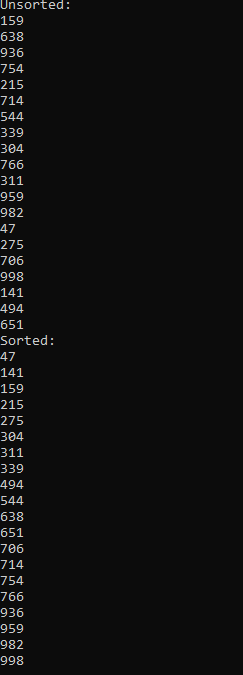
\includegraphics[]{quickSort.png}
    \subsection{Bucket Sort}
    \textbf{Note: Did file redirection to get output for bucket sort since its too large for screen shot}
Unsorted:
823
\\368
\\269
\\387
\\308
\\653
\\283
\\420
\\310
\\780
\\678
\\126
\\134
\\412
\\239
\\366
\\349
\\106
\\356
\\380
\\688
\\595
\\338
\\542
\\488
\\230
\\223
\\800
\\86
\\350
\\782
\\909
\\718
\\404
\\649
\\26
\\57
\\932
\\799
\\719
\\64
\\477
\\846
\\198
\\241
\\437
\\917
\\590
\\543
\\273
\\323
\\583
\\221
\\661
\\125
\\709
\\243
\\700
\\861
\\330
\\51
\\996
\\239
\\121
\\400
\\240
\\500
\\809
\\173
\\651
\\881
\\589
\\480
\\79
\\788
\\722
\\516
\\705
\\664
\\411
\\330
\\339
\\346
\\551
\\353
\\824
\\260
\\596
\\524
\\474
\\926
\\575
\\470
\\518
\\49
\\870
\\758
\\549
\\31
\\283
\\Sorted:
\\26
\\31
\\49
\\51
\\57
\\64
\\79
\\86
\\106
\\121
\\125
\\126
\\134
\\173
\\198
\\221
\\223
\\230
\\239
\\239
\\240
\\241
\\243
\\260
\\269
\\273
\\283
\\283
\\308
\\310
\\323
\\330
\\330
\\338
\\339
\\346
\\349
\\350
\\353
\\356
\\366
\\368
\\380
\\387
\\400
\\404
\\411
\\412
\\420
\\437
\\470
\\474
\\477
\\480
\\488
\\500
\\516
\\518
\\524
\\542
\\543
\\549
\\551
\\575
\\583
\\589
\\590
\\595
\\596
\\649
\\651
\\653
\\661
\\664
\\678
\\688
\\700
\\705
\\709
\\718
\\719
\\722
\\758
\\780
\\782
\\788
\\799
\\800
\\809
\\823
\\824
\\846
\\861
\\870
\\881
\\909
\\917
\\926
\\932
\\996

\end{document}